\documentclass{jsarticle}
\usepackage[dvips]{graphicx}
\usepackage{comment}
\setlength{\textheight}{24cm}
\setlength{\topmargin}{-1.5cm}
\setlength{\textwidth}{17cm}
\setlength{\oddsidemargin}{-.5cm}

%
% 演習課題レポートの番号,氏名(学番号),提出日を明記すること.
%
\title{エージェント工学:第1回レポート課題}
\author{澤 \/ 祐里(21--1--037--0801)} % 氏名(学番号)
\date{\today} % 提出期限(厳守) 

\begin{document}
\maketitle

\section{人生設計}
\subsection{自分の目的とすること}
私は、私が小さい時から人が苦手で、人と直接関わらなくても楽しめるゲームばっかりやって
きました。しかし、その生活ができるのは親がお金を稼いでくれているからであり、
これから先の将来は自分でお金を稼ぐ必要があるため、その生活をやめなければいけない。
その中で、私は「苦手な人と直接関わらずにやりたいことをして生きていく」という欲求を満たすため、
人と直接関わらずにお金を稼ぐ手段を見つけた上で、そのお金だけで生きていけるようにする
必要がある。しかし、現実的に考えると一人でお金を稼いでいくのは難しいため、
あまり人と関わらなくても自由にすごせるぐらいの収入を得られる方法を見つけて
、他人やお金に縛られずに自由に生きていくことを人生の目的とする。
\subsection{自分のやりたいこと}
\begin{itemize}
  \item 田舎に大きな家を立てて、そこで身内だけを集めて遊びたい。
  \item 自分で考えた大きなゲームを作りたい。
  \item 常に新しいことに挑戦したい。
\end{itemize}

\section{目的を達成する方法}
自分の目的に一番近いものが、不労所得だけで食べていけるようにすることだと考えており、
それを実現させるためには、豊富な資産や不労所得のシステムを作れるスキルが必要になると考えているため
、まずは、それらを得るために一般の企業に就職することを目標にする。
様々な業種が存在する中で、私は不労所得を作るなら、コンピューターに代わりに仕事をさせることができる
IT系だと考えているため、IT系の企業に就職したいと考えている。そして、特にIT系の中でも、自分がプログラミングが
好きであるため、プログラマーかそれに準ずる職業に就きたいと考えている。
また、IT系の仕事はインターネットを利用することで、人と直接関わらず仕事ができるテレワークなどが
可能であったりするため、私の目的に合致している。
自分のやりたいことをすべて実現するためには、経済的な余裕と時間が必要なので、継続的に貯金していく。

\section{目標を達成するためにやっていること・やるべきこと}
\subsection{現在指向的意図}
現在指向的意図として、プログラミングと英語の勉強がある。
プログラミングは自分が好きなことであり、プログラミングは毎日やれば、どんどんできることが
増えていく上に、それを仕事に活かすこともできるため
、日頃からプログラミングに触れるようにしている。
具体的には、Unityで自分で考えたアイデアと既存のゲームを組み合わせた
新しいゲームを1から自分で作成したり、
GANなどの新しい技術をPythonで動かしてみて遊んだりしている。
将来的には、これらを発展させて、例えばスマホゲームを作ったり、最新の技術を紹介する動画
クリエイターとして収益化を狙いたいと考えている。
英語の勉強は、GANなどに始まる新しい研究の情報はインターネット上に沢山でているが、
そのほとんどが英語で書かれており、日本語の文献が非常に
少ないため、新しいことを学んだりするには、英語力があった方がとても有利に働くと考えているため、
英語力をつけるためにTOEIC勉強のアプリを使って、TOEICの勉強を毎日するようにしている。
\subsection{未来指向的意図}
未来指向的意図として、TOEICの受験、IT系企業のインターンシップ、就職活動がある。
TOEICの受験は、私がTOEICの勉強をしていることに加えて、
単純に私がプログラマーには英語力が必要だと考えているのもあり、
TOEICのスコアが高ければ、就職活動の際に有利になると思っているため、
10月に近畿大学で開催予定のTOEICを受けようと考えている。
IT系企業のインターンシップは、私が企業に就職した際に具体的にどのような仕事をするのかを
知ることで、自分の目的にあったスキルが手に入るのかを確かめたいという考えと、就職活動で
プラスになるんじゃないかという考えの元で、IT系の業種という広い枠組みで、
できる限り沢山の企業にインターンシップの申し込みをしようと思っている。
就職活動は、とりあえず今の内からでもできることは始めていこうと考えており、自己PRに必要な
自分の長所や短所などの自分の情報をメモ帳などに書き出したりして自己分析をしておいたり、
SPIの対策として、ネットに上がっているSPIの問題を解いていく、動画サイトに上がっている
SPIの解き方の動画などを視聴してSPIの対策について学ぶことなど
を今年の内から始めておきたいと考えている。他にも、自分が人が苦手というのもあって、
面接が不安要素なので、友達や教授の協力をいただいて、面接の練習を早くから行うなどを
考えている。自分がやりたいことが多いために、エントリー前に優柔不断になって会社を選べない
という事態にならないように、
今年中には、インターンシップや会社説明、口コミサイトなどの情報をもとにして、
どこの会社に入るかの候補を10社くらいまで絞り込んで、会社のエントリーも迷わずできるよう
な状態にまで持っていき、就職活動は早々に終わらせたいと考えている。


\begin{figure}[b]
  \begin{center}
  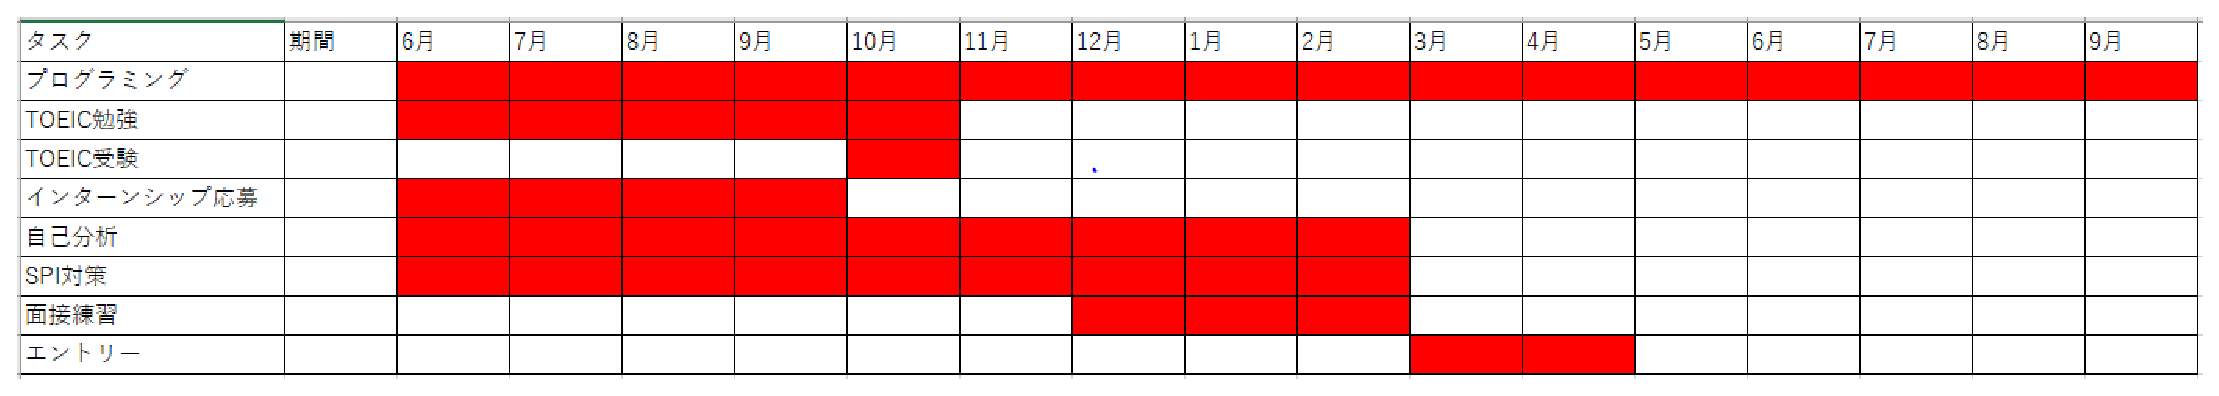
\includegraphics[scale=0.5]{1.eps}
  \caption{ガントチャート
  }
  \label{fig:1}
  \end{center}
\end{figure}

\end{document}

